%%% LaTeX Template: Two column article
%%%
%%% Source: http://www.howtotex.com/
%%% Feel free to distribute this template, but please keep to referal to http://www.howtotex.com/ here.
%%% Date: February 2011

%%% Preamble
\documentclass[	DIV=calc,%
							paper=a4,%
							fontsize=12pt,%
							onecolumn]{scrartcl}	 					% KOMA-article class

\usepackage{lipsum}													% Package to create dummy text
\usepackage[english]{babel}										% English language/hyphenation
\usepackage[protrusion=true,expansion=true]{microtype}				% Better typography
\usepackage{amsmath,amsfonts,amsthm}					% Math packages
\usepackage[pdftex]{graphicx}									% Enable pdflatex
\usepackage[svgnames]{xcolor}									% Enabling colors by their 'svgnames'
\usepackage[hang, small,labelfont=bf,up,textfont=it,up]{caption}	% Custom captions under/above floats
\usepackage{epstopdf}												% Converts .eps to .pdf
\usepackage{subfig}													% Subfigures
\usepackage{booktabs}												% Nicer tables
\usepackage{fix-cm}													% Custom fontsizes
\usepackage[utf8]{inputenc}
\usepackage[top=2.5cm, bottom=2.5cm, left=2.5cm, right=2.5cm]{geometry}
\usepackage[ddmmyyyy]{datetime}
\addto\captionsenglish{%
	\renewcommand\tablename{Tabela}
	\renewcommand\figurename{Figura}
} 
 

 
%%% Custom sectioning (sectsty package)
\usepackage{sectsty}													% Custom sectioning (see below)
\allsectionsfont{%															% Change font of al section commands
	\usefont{OT1}{phv}{b}{n}%										% bch-b-n: CharterBT-Bold font
	}

\sectionfont{%																% Change font of \section command
	\usefont{OT1}{phv}{b}{n}%										% bch-b-n: CharterBT-Bold font
	}



%%% Headers and footers
\usepackage{fancyhdr}												% Needed to define custom headers/footers
	\pagestyle{fancy}														% Enabling the custom headers/footers
\usepackage{lastpage}	

% Header (empty)
\lhead{}
\chead{}
\rhead{}
% Footer (you may change this to your own needs)

%% ====================================
%% ====================================
%% mude o rodape  do projeto
%% ====================================
%% ====================================

\lfoot{\footnotesize \texttt{Etech Prestadora de Serviços - (43)999980797} \textbullet ~ Londrina / Pr.}


\cfoot{}
\rfoot{\footnotesize página \thepage\ de \pageref{LastPage}}	% "Page 1 of 2"
\renewcommand{\headrulewidth}{0.0pt}
\renewcommand{\footrulewidth}{0.4pt}



%%% Creating an initial of the very first character of the content
\usepackage{lettrine}
\newcommand{\initial}[1]{%
     \lettrine[lines=3,lhang=0.3,nindent=0em]{
     				\color{DarkGoldenrod}
     				{\textsf{#1}}}{}}



%%% Title, author and date metadata
\usepackage{titling}															% For custom titles

\newcommand{\HorRule}{\color{DarkGoldenrod}%			% Creating a horizontal rule
									  	\rule{\linewidth}{1pt}%
										}

\pretitle{\vspace{-12pt} \begin{flushleft} \HorRule 
				\fontsize{24}{24} \usefont{OT1}{phv}{b}{n} \color{DarkRed} \selectfont 
				}

%% ====================================
%% ====================================
%% mude o titulo  do projeto
%% ====================================
%% ====================================

\title{Projeto de cabeamento estruturado da empresa Etech ISP}					% Title of your article goes here

%% ====================================



\posttitle{\par\end{flushleft}\vskip 0.5em}

\preauthor{\begin{flushleft}
					\large \lineskip 0.5em \usefont{OT1}{phv}{b}{sl} \color{DarkRed}}
\author{André Giuliani RA 1909797 }  	% Author name goes here


\postauthor{\footnotesize \usefont{OT1}{phv}{m}{sl} \color{Black} 
					\\Universidade Tecnológica Federal do Paraná - Campus Cornélio Procópio
					\\Pós Graduação - Disciplina de Redes Estruturadas 								% Institution of author
					\par\end{flushleft}\HorRule}

\date{}																				% No date




%%% Begin document
\begin{document}
\maketitle
\thispagestyle{fancy} 	
\thispagestyle{empty}		% Enabling the custom headers/footers for the first page 
% The first character should be within \initial{}




%% ====================================
%% ====================================
%% mude o resumo  do projeto
%% ====================================
%% ====================================
\initial{E}\textbf
{	ste projeto visa atender a empresa de telecomunicações Etech ME no que se refere à estrutura interna para a rede lógica, esta rede compreenderá serviços de dados (Computadores e Servidores), voz (Telefones IP) e monitoramento de imagem (Cftv/IP). Trata-se de uma instalação nova sendo que no local ainda não há nenhuma infraestrutura pronta. Todos os pontos descritos serão atendidos cabos de rede Cat 6 que possuem capacidade de transmissão de até 10GBps, após a instalação todos os pontos serão aferidos pelo processo de certificação.}\\

\textbf
{	Conforme levantamento no local, junto aos sócios, a empresa está iniciando seus trabalhos como um pequeno provedor de internet via fibra no bairro Vila Casone em Londrina Pr., porém, apesar da estrutura inicial ser considerada pequena o projeto deverá contemplar futuras ampliações evitando custos desnecessários a posteriori; as futuras ampliações se limitarão ao patamar de duas vezes o tamanho da rede inicialmente implantada e deverão ser aplicadas a todos os passivos de rede pertinentes, tais como: Eletrocalhas, dutos, racks, quadros etc.}

%% ====================================
\begin{figure}
	\centering
	
\includegraphics{Etech}
\end{figure}

\vspace{3cm}
\centerline{\textit{\textbf{\today}}}

\clearpage
    \renewcommand*\listfigurename{Lista de figuras}
\listoffigures

\renewcommand*\listtablename{Lista de tabelas}
\listoftables




\clearpage
\renewcommand{\contentsname}{Sumário}
\tableofcontents
\clearpage

%% ====================================
%% ====================================
%% Inicio do texto
%% ====================================
%% ====================================
\section{Introdução}

%Explique nesta primeira seção qual seria o perfil do caso. Perfil do cliente, quantidade de colaboradores, quantidade de equipamentos de TI atualmente
Este projeto de cabeamento estruturado destina-se à empresa Etech ISP, trata-se de um provedor de pequena escala de serviços de comunicação multimídia e acesso á internet. Será executado a instalação de 10 pontos de rede em um prédio recém construído pela empresa. Inicialmente a empresa conta com 5 colaboradores sendo 3 da área técnica, 1 administrativos e 1 comercial, cada colaborador utilizará em seu posto de trabalho um desktop e um telefone IP. Atualmente os recursos ativos de TI constam de:
Desktop Dell: 5 unidades;
Telefones IP Intelbrás: 6 unidades;
Servidor Dell: 1 unidade (No servidor estão virtualizados os serviços de Banco de dados, Aplicativo gerencial e Pabx IP); 
%Indique também nesta seção o escopo do projeto.
O propósito deste projeto é montar uma rede interna de alta capacidade e confiabilidade, com possibilidade de expansões futuras na proporção de 2 vezes o tamanho original.
%Apresente um overview do parque tecnológico do caso.


\subsection{Benefícios}
%Explique quais seriam os benefícios provenientes da execução deste projeto.
O sistema de cabeamento estruturado visa padronizar as instalações referentes a conectividade, trata-se de uma solução estratégica pois miniminiza custos de uma readequação física para mudanças de local no trabalho ou mesmo de novas instalações, segue os principais benefícios que a rede estruturada irá proporcionar:
\begin{itemize}
\item Suporte a diversos padrões de comunicação que utilizarão o mesmo meio físico, neste caso os sistemas de informática, telefonia e segurança irão utilizar o mesmo meio físico bem como o mesmo meio lógico utilizando o protocolo IP.
\item Facilidade na mudança de layout interno visto que as interfaces são padronizadas e os equipamentos portam suas respectivas configurações \item independente que qual local estejam conectados na rede.
\item Manutenção simples e rápida uma vez que todos os cabos e dispositivos são organizados e identificados em ambas extremidades.
\item Localização fácil de um cabo devido ao mesmo ser identificado por todo seu trajeto.
\item Documentação técnica que facilita a manutenção e novas implantações.
\end{itemize}
 
\section{Estado atual}

%Aprente o estado atual da rede. Caso não tenha rede, desconsiderar esta seção.
Atualmente a empresa é uma prestadora de serviços na área telemática e encontra-se em uma edícula que está atrás do novo prédio construído para abrigar a nova sede e os novos serviços, logo não será reaproveitado nenhum material, exceto os computadores e telefones IP utilizados atualmente.\\
Os passivos de rede, tais como pacth panel e cordões, não serão utilizados uma vez que são de categoria inferior à que será adotada na nova sede. Os passivos atuais são CAT 5E e a nova rede será CAT6.


%Caso tenha rede, deixe claro:
%os passivos de rede atuais:path panels, cabos, etc..;
%as principais reclamações dos usuários. Qual o principal motivo da reestruturação? Efetue uma pesquisa junto aos colaboradores para determinar quais problemas a rede apresenta.
%Observações. Analise a rede e verifique se há estruturas que não se enquadram nas normas ou que indicam suspeita de problemas.



\section{Usuários e Aplicativos}
%Explique nesta seção os usuários atuais e o perfil de crescimento, se por exemplo, há estimativa na evolução da empresa no que tange a quantidade de usuários, pontos de redes, equipamentos.
Hoje a equipe conta com 5 colaboradores divididos entre técnicos, administrativos, comercial e diretoria, há uma expectativa de triplicar este efetivo, porém isto se dará de acordo com o crescimento do provedor.\\
A empresa Etech Instaladora continuará a existir em concomitância com a Etech ISP será utilizado a mesma infraestrutura interna de TI.
 

\subsection{Usuários}
%Crie uma relação da quantidade, perfil de usuários de seu projeto.

Os usuários da empresa dividem-se me 3 grupos: Departamento técnico, administrativo e comercial.
Apenas o departamento técnico terá acesso irrestrito (e controlado) a todos os sistemas da empresa, os demais usuários terão acesso apenas aos serviços pertinentes à sua atuação profissional.


\subsection{Aplicativos}
%Crie uma relação dos aplicativos e seus níveis críticos de uso.
Os aplicativos referentes à administração serão hospedados em um servidor virtual que será dividido da seguinte forma:\\

\begin{itemize}
\item Servidor de Banco de Dados: Este servidor abrigará todos os dados gerenciais da empresa, tais como base de clientes, financeiro e dados administrativos entre outros que se referem à administração geral do negócio. Ficará oculto na rede e somente será acessado pelo servidor de aplicação (WEB) utilizando do modelo de 3 camadas;
\item Servidor de aplicação: Este servidor será responsável por fazer a ponte entre o banco de dados e a interface Web com o usuário. Como todo o sistema de gerenciamento é via WEB nas máquinas dos usuários não haverá nenhuma aplicação que requeira um desempenho muito alto de rede.
\item Servidor (Gerência de rede). Este servidor irá gerenciar a parte de acesso à internet dos clientes do provedor ISP. Este servidor, embora esteja na mesma rede interna, será acessado apenas pelo departamento técnico em uma Vlan exclusiva para este serviço. Este servidor requer que um software "Cliente" seja instalado na máquina do colaborador, estas gerências requerem um pouco mais de processamento porém nada que cause grande impacto na rede. Nas máquinas que receberão este software cliente deverá ser instalado um adaptador de rede que comporte o uso de Lan virtuais Vlan. 

\end{itemize}


\section{Estrutura predial existente}

%Explique aqui a planta física dos prédios
%Pode ser anexada, em escala ou não.

Segue a planta física da nova sede. Trata-se de um prédio inicialmente com 40m2 de construção com um escritório, uma recepção, área de produção e uma sala de telecomunicações onde serão abrigados os equipamentos de TI da empresa.

\begin{figure}
	\centering
	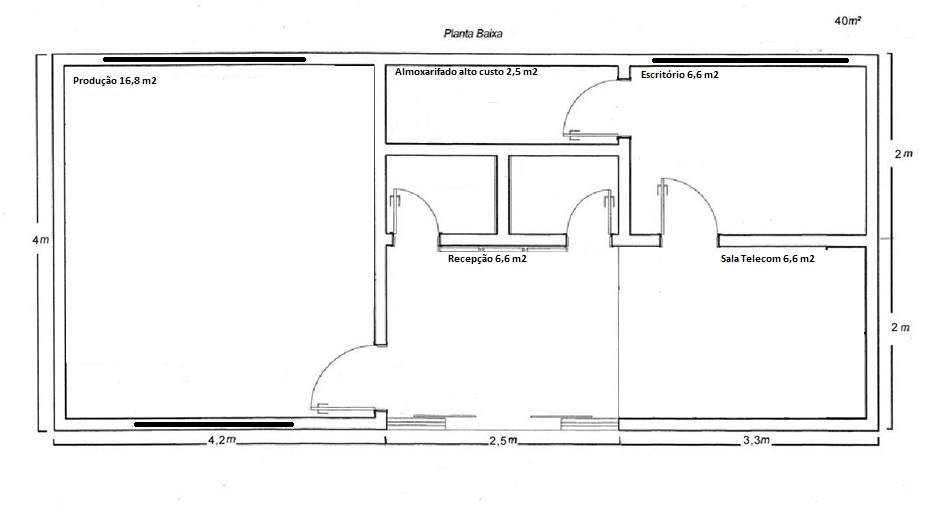
\includegraphics[width=\textwidth]{fig4}
	\caption{Planta baixa sem escala}
	\label{fig4}
\end{figure}

%Deve conter uma descrição geral, indicando a possível distância entre os pontos de rede e restrições de instalação.
Por tratar-se de um local com dimensões reduzidas está descartada a preocupação com distancia dos cabos, tendo em vista que o cabo mais longo terá aproximadamente 15 metros lineares. 
O espaço da sala de telecomunicações está equipado com piso elevado, o que facilita a manutenção e novas implementações.


\section{Planta Lógica - Elementos estruturados}

\begin{figure}
	\centering
	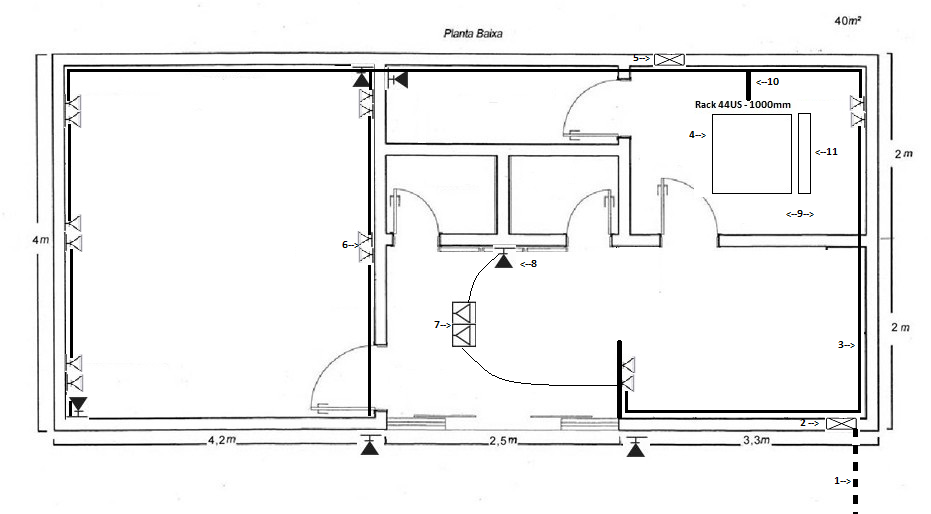
\includegraphics[width=\textwidth]{fig5}
	\caption{Planta implantação sem escala}
	\label{fig5}
\end{figure}

\subsection{Estado atual}
%Deve ter a planta atual, se for o caso
Atualmente o novo prédio não está terminado e a perspectiva para sua ocupação é para 120 dias.
Conforme visto na figura acima houve a necessidade do TI modificar o lay-out original do prédio.

\subsection{Topologia}

Adendos do projeto conforme a figura 5:\\

1- \textbf{Entrance Facility (EF)}: Trata-se da entrada de serviços de telecomunicações. Trata-se de uma tubulação de PVC que será anexada ao poste de entrada do cliente por onde entrarão os serviços de voz (Linhas telefônicas) e internet (link entrada de internet). Por esta tubulação também passarão dois cabos de 4 fibras que atenderão os clientes da empresa.\\
2- \textbf{DG de Telecom}: Trata-se de uma caixa embutida na parede que faz parte da EF. Esta caixa isola a rede interna do cliente da rede externa da operadora e serve para delimitar suas responsabilidades sobre os serviços.\\
3- \textbf{Horizontal Cabling}: Refere-se à distribuição interna dos cabos. A distribuição interna se dá por meio de eletrocalhas fixadas próximas aos limites superiores do pé direito da edificação e ficarão o mais próximo possível das paredes.\\ 
4- \textbf{Equipament Room (ER)}: Devido ao espaço físico ser limitado o (ER) compartilha a mesma sala do Telecommunications Room (TR). Neste caso o (ER) será um rack de 44US que comportará dois servidores, uma OLT de Gpon e um roteador que levará internet aos clientes da empresa.\\
5- \textbf{Quadro de distribuição elétrica exclusivo da (TR) e (ER)}: Trata-se de um quadro definido em projeto elétrico anexo onde o mesmo fará a distribuição isolada da rede elétrica para cada equipamento bem como proverá backup elétrico nos casos de falha ne rede elétrica da concessionária de energia.\\
6- \textbf{Mutoa}: Trata-se da interligação final do cabeamento com o equipamento do cliente. Todas as Mutoas do item 6, com exceção da sala da recepção e câmeras, serão do tipo sobrepor, fixadas na parede, com duas saídas para conectores fêmeas RJ45. A altura em relação ao piso é de 30 cm.\\
7- \textbf{Mutoa}: A Mutoa do item 7 é do tipo de embutir no piso com 2 saídas para conectores fêmea RJ45. Deverá prover proteção quanto a impactos e entrada de água.\\
8- \textbf{Mutoa}: A Mutoa do item 8 segue as especificações do item 6, porém com a diferença de abrigar somente 1 conector fêmea RJ45 e estar a 2,5 mts de altura em relação ao piso.\\
9- \textbf{Equipament Room (ER)}: Sala de equipamentos com piso elevado.
10- Descida da eletrocalha para o rack.\\
11- \textbf{Telecommunications Room (TR)}: Compartilha o mesmo espaço físico da (ER). Nesta sala encontra-se o Bracket que é um rack aberto onde todoas os cabos são organizados e conectados às suas respectivas redes.\\
12- \textbf{Work Área (WA)}: A (WA) é onde ocorre a produção propriamente dita da empresa. Neste caso a (WA) possui um escritório com cinco possibilidades de interligação à rede (Mesas), uma recepção e uma sala da diretoria.\\
14- \textbf{Backbone Cabling}: Trata-se da interligação das salas de (ER)e (TR). Neste caso será a interligação do rack de servidores com o Bracket da distribuição horizontal. Neste caso haverão dois Pacth Panels CAT6 com 6 cabos fazendo esta interconexão.\\
 

%Proposta futura, proposta após implantação.
%Deve conter o diagrama da rede. Atente-se a redundância  e ligações truncadas.
%Deve explicar todos termos e componentes utilizados nestas plantas. Por exemplo: entrance facility, work area, horizontal cabling, etc..
%Todos os elementos das figuras devem ser explicados. 
%Crie esboço da configuração dos racks e brackets. Explique cada um dos componentes. Você pode criar uma tabela contendo figuras dentro, ou criar uma tabela e incluí-la como imagem. Por exemplo, verifique a tabela \ref{tab1}.

\subsection{Encaminhamento}
%Eletrodutos, calhas, e qualquer material em que os cabos serão alojados/alocados.
Grande parte do Cabeamento Horizontal seguirá da (TR) até a Mutoa via eletrocalha aérea e aparente. Em cada ponto final de conexão o cabo sairá da eletrocalha e descerá até a Mutoa por um conduíte de aço galvanizado pintado eletrostaticamente na cor areia. Este tubo interligará a eletrocalha até a Mutoa que estará abrigada em um condulete de antimônio na medida de 4x2". 

\subsection{Memorial descritivo}

%Relacione todos os equipamentos passivos que serão utilizados, tipo, fabricante, quantidade.
\begin{table}[h!]
\centering
\caption{Memorial Descritivo}
\label{Memorial Descritivo}
\begin{tabular}{|l|l|l|l|l|}
\hline
QTD & UNID & DESCRICAO                     & MARCA / MODELO          & ITEM \\ \hline
01  & PC   & Rack piso 44US x 1000mm       & Attic AS-Server         & 1    \\ \hline
01  & PC   & Rack piso tipo Bracket        & Attic OP-Rack           & 2    \\ \hline
30  & PC   & Eletrocalha 50x50x3000mm      & H-Leve - Perfurada      & 3    \\ \hline
30  & PC   & Gancho Sustentação EletroC    & H-Leve - N.A.           & 4    \\ \hline
5   & PC   & Curva 90 aberta 50x50         & H-Leve - Interna        & 5    \\ \hline
2   & PC   & Curva Vertical 50x50          & H-Leve - Externa        & 6    \\ \hline
15  & PC   & Condulete 4x2 Sobrepor        & Daísa - 1 saída         & 7    \\ \hline
7   & PC   & Mutoa 2 saídas RJ45           & Daísa - 2 Saídas        & 8    \\ \hline
7   & PC   & Mutoa 1 Saída RJ45            & Daísa - 1 Saída         & 9    \\ \hline
1   & PC   & Caixa Piso 4x4                & Wetzel - A4-1           & 10   \\ \hline
1   & PC   & Mutoa 2 saídas 4x4 blindada   & Wetzel - 2RJ45          & 11   \\ \hline
7   & PC   & Tubos 1"x3M Galvanizado       & Zetone - Pintura Eletro & 12   \\ \hline
7   & PC   & Saída Horizontal Eletrocalha  & Zetone - 1"             & 13   \\ \hline
21  & PC   & Conector RJ45 Fêmea CAT6A     & Furukawa - GigaLan      & 14   \\ \hline
3   & PC   & Pacth Panel CAT6A             & Furukawa - GigaLan      & 15   \\ \hline
2   & CX   & Cabo Rede CAT6A Vermelho      & Furukawa - Gigalan      & 16   \\ \hline
22  & PC   & Line Cord CAT6A Vermelho      & Furukawa - Gigalan      & 17   \\ \hline
14  & PC   & Line Cord CAT6A Verde         & Furukawa - Gigalan      & 18   \\ \hline
14  & PC   & Line Cord CAT6A Amarelo       & Furukawa - Gigalan      & 19   \\ \hline
3   & PC   & Fita para Rotuladora          & Brother - Branca        & 20   \\ \hline
3   & PC   & Bandeja Rack 4x4 Corrediça    & Attic - 1000mm Vent     & 21   \\ \hline
5   & PC   & Guia Cabo Rack 1U             & Attic - 1UFix           & 22   \\ \hline
1   & PC   & Kit Ventilação Rack 4 Coolers & Attic - Cooler          & 23   \\ \hline
3   & PC   & Régua Elétrica para Rack      & Attic - 12 Tomadas      & 24   \\ \hline
10  & MT   & Fita Velcro Dupla Face        & Genérico                & 25   \\ \hline
1   & PC   & Kit 100 Pçs Parafuso e Porca  & Genérico                & 26   \\ \hline
1   & PC   & DG Telecom Telebras 800x800   & Engelco - Embutido      & 27   \\ \hline
2   & PC   & Bloco Telecom M10             & Bargoa - M10            & 28   \\ \hline
4   & PC   & Anel Guia DG Nr 6             & Genérico                & 29   \\ \hline
\end{tabular}
\end{table}


\subsection{Identificação dos cabos}
%llll
Todos os cabos instalados bem como os line cords dos lados A e B serão identificados, inclusive durante seu trajeto, com etiquetas plásticas brancas de 12mm. As etiquetas serão  impressas em rotuladora térmica com fonte preta e seguirão a normativa NBR 14565.
Devido ao porte, este projeto utilizará apenas o item 1 da tabela de identificação (PT XX XXX), onde PT indica que é um ponto de telecomunicações (Rede), XX será 01 tendo em vista que só há um pavimento e XXX irá de 001 até 024 que é a quantidade de cabos utilizados.
A figura abaixo exemplifica o modelo de identificação:

\begin{figure}[h!]
	\centering
	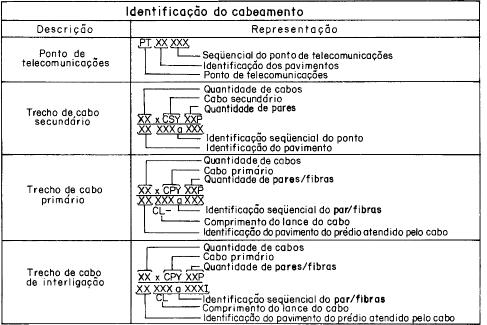
\includegraphics[width=\textwidth]{fig6}
	\caption{Modelo de Identificação}
	\label{fig6}
\end{figure}



\section{Implantação}
%Estabeleça um cronograma de implantação:
%Remoção de equipamentos existentes (destino para descarte), instalação dos condutores, instalação dos cabos, 
%identificação dos cabos, montagem dos racks, certificação, etc... Crie atividades e estabeleça o tempo de execução. Se for um projeto real, indique também quais os responsáveis pela execução do projeto e de cada uma das etapas.

%Defina marcas (e padrões) e fornecedores se for o caso. Atenção a contratados e subcontratados para a realização das atividades. Estabeleça a responsabilidade de execução da atividade e também da validação dela.

%Utilize algum software para gerear o cronograma. Excel,etc. O fundamental é dividir em etapas, descrever e estimar o tempo de cada uma delas.

%Segue uma relação de ferramentas:
%http://asana.com/, 
%https://trello.com/, 
%http://www.ganttproject.biz/, 
%http://www.orangescrum.org/. 

\section{Plano de certificação}

A certificação ocorrerá após a total instalação e conectorização dos cabos devendo esta ser executada em até 1 dia após a conclusão da instalação.\\
A certificação ocorrerá na forma passiva e será utilizado o certificador Fluke DTX1500 que atende a especificação \textbf{CAT6A 1000Base-TX}, após a conclusão será emitido o laudo impresso referente a avaliação executada bem como os resultados obtidos.\\
Uma vez que os Line Cords (Pacth Cords) já vêm certificados pelo fabricante a certificação coletará dados do "Link Permanente", ou seja, a rede que sai da tomada fêmea do ponto final até o Pacth Panel que está instalado na Telecommunications Room (TR). 
%Quais seriam as etapas para a certificação? 
%Quais os locais e horários para execução da certificação na rede? Toda rede será certificada?
%Como os testes seriam executados?
%Quais relatórios de certificação serão (ou deveriam ser) entregues? 
%Revisões periódicas na rede, emissão de certificados para novos pontos.
\section{Plano de manutenção}

Estão previstas 4 manutenções preventivas durante o período de garantia da mão de obra sobre a instalação. Estas revisões constam de inspeção visual de toda a rede bem como testes ativos (Com a rede em produção)tais como ping. latência, erros de CRC entre outros. Os testes passivos serão executados com o o TestSet TSW900ETH da Wise Ind. que visa estressar a rede com a máxima taxa de transferência possível com a finalidade de coletar dados sobre sua integridade. Os dados aferidos pelo TestSet serão impressos e entregue ao cliente. Os dados aferidos são

\begin{table}[h!]
\centering
\caption{Testes Manutenção Preventiva}
\label{my-label}
\begin{tabular}{ll}
Trafego                                    & Ate o limite tecnico especificado no IEEE 802.3               \\
Trafego                                    & Com tamanho fixo e variado                                    \\
Gerar e medir                              & Quadros menores ou maiores que o especif.  pelo IEEE 802.3    \\
Gerar e medir                              & Erros de CRC                                                  \\
Medir                                      & Quadros e Bytes Transmitidos e Recebidos                      \\
Medir                                      & Quadros Fragmentados                                          \\
Medir                                      & Quadros sem sequencia                                         \\
Medir                                      & Colisoes                                                      \\
Medir                                      & Throughput (RFC2544)                                          \\
Medir                                      & Delay (RFC 2544)                                              \\
Medir                                      & Perda de Pacotes (RFC2544)                                    \\
Medir                                      & Back-to-back frames (RFC 2544)                                \\
Gerar e medir                              & BERT                                                          \\  
\end{tabular}
\end{table}



\subsection{Plano de expansão}
%Existe um plano de expansão? Quantos novos pontos poderão ser acrecidos na rede, antes de migração de equipamentos na camada 2? Se houver expansão, quais equipamentos deverão ser direcionados para as estremidades da rede? 
Conforme visto no início deste projeto há uma previsão de ampliação de rede na proporção máxima de duas vezes (1 + 1) o tamanho atual.\\
Os dutos e eletrocalhas já estão preparados para esta possível expansão bastando apenas integrar os novos caminhos aos já existentes. No Bracket também há espaço reservado para esta possibilidade, bastando adicionar novos Pacth Panel's conforme a necessidade e um novo Switch caso sejam necessários mais de 48 portas elétricas.\\
Para manter a homogeneidade e a qualidade da rede deverão ser utilizados preferencialmente as mesmas marcas e modelos dos materiais já aplicados, caso já estejam fora de linha deverão ser utilizados materiais e equipamentos que excedam as especificações dos atuais. 

\section{Orçamento}
%Crie uma relação de orçamentos baseado na seções anteriores.
Os investimentos necessários para a implementação do que foi descrito até aqui segue na tabela abaixo. Lembrando que obras de alvenaria não estão incluídas na mão de obra e mudanças de layout serão avaliadas a parte deste orçamento.

\begin{table}[h!]
\centering
\caption{Investimento}
\label{my-label}
\begin{tabular}{|c|c|c|c|}
\hline
ITEM         & QTD   & VL UNIT      & VL TOTAL      \\ \hline
1            & 1     & R\$ 2.500,00 & R\$ 2.500,00  \\ \hline
2            & 1     & R\$ 1.250,00 & R\$ 1.250,00  \\ \hline
3            & 30    & R\$ 37,00    & R\$ 1.110,00  \\ \hline
4            & 30    & R\$ 3,00     & R\$ 90,00     \\ \hline
5            & 5     & R\$ 17,00    & R\$ 85,00     \\ \hline
6            & 2     & R\$ 18,00    & R\$ 36,00     \\ \hline
7            & 15    & R\$ 12,00    & R\$ 180,00    \\ \hline
8            & 7     & R\$ 6,00     & R\$ 42,00     \\ \hline
9            & 7     & R\$ 6,00     & R\$ 42,00     \\ \hline
10           & 1     & R\$ 12,00    & R\$ 12,00     \\ \hline
11           & 1     & R\$ 27,00    & R\$ 27,00     \\ \hline
12           & 7     & R\$ 26,00    & R\$ 182,00    \\ \hline
13           & 7     & R\$ 3,00     & R\$ 21,00     \\ \hline
14           & 21    & R\$ 30,00    & R\$ 630,00    \\ \hline
15           & 3     & R\$ 440,00   & R\$ 1.320,00  \\ \hline
16           & 2     & R\$ 898,00   & R\$ 1.796,00  \\ \hline
17           & 22    & R\$ 22,00    & R\$ 484,00    \\ \hline
18           & 14    & R\$ 22,00    & R\$ 308,00    \\ \hline
19           & 14    & R\$ 22,00    & R\$ 308,00    \\ \hline
20           & 3     & R\$ 42,00    & R\$ 126,00    \\ \hline
21           & 3     & R\$ 150,00   & R\$ 450,00    \\ \hline
22           & 5     & R\$ 25,00    & R\$ 125,00    \\ \hline
23           & 1     & R\$ 189,00   & R\$ 189,00    \\ \hline
24           & 1     & R\$ 95,00    & R\$ 95,00     \\ \hline
25           & 10    & R\$ 12,00    & R\$ 120,00    \\ \hline
26           & 1     & R\$ 100,00   & R\$ 100,00    \\ \hline
27           & 1     & R\$ 230,00   & R\$ 230,00    \\ \hline
28           & 1     & R\$ 35,00    & R\$ 35,00     \\ \hline
29           & 1     & R\$ 4,00     & R\$ 4,00      \\ \hline
TOTAL        &       &              & R\$ 11.897,00 \\ \hline
MÃO DE OBRA  &       &              & R\$ 7.350,00  \\ \hline
CERTIFICAÇÃO & 24    & PONTOS       & R\$ 1.500,00  \\ \hline
             &       &              &               \\ \hline
VALOR        & FINAL &              & R\$ 20.747,00 \\ \hline
\end{tabular}
\end{table}

\section{Referências bibliográficas}
%Utilize o mendley, o jabref ou diretamente o bibtex para gerenciar suas referências biliográficas. As referências são criadas automaticamente de acordo com o uso no texto.

%Exemplo: Redes de computadores, segundo \cite{t2013} é considerada..... Já \cite{kurose2010} apresenta uma versão...

%Analisando os pressupostos de \cite{ref3} e \cite{ref4} concluimos que....


\renewcommand\refname{} %%Referências bibliográficas}  
\bibliographystyle{ieeetr}
\bibliography{referencias}  

%% ***********************************************************************
%% === remover daqui =====================================================
%% ***********************************************************************

%\section{Elementos textuais - Alguns exemplos}

%Esta seção apresenta exemplos de elementos textuais. \textbf{Remova-a da versão final do texto}.


%\subsection{Colocar elementos em itens}

%Texto antes da lista

%\begin{itemize}
%	\item First item in a list 
%	\item Second item in a list 
%	\item Third item in a list
%\end{itemize}

%\subsubsection{Uma sub seçao de terceiro nivel}

%Exemplo de uma subseção
%
%\subsection{Tabelas}

%Utilize o site http://www.tablesgenerator.com/ para elaborar as tabelas de seu trabalho.
%Para adicionar uma tabela utilize: a tag input, passando o arquivo da tabela como parametro

%\begin{table}[h!] % coloque h! para forcar a posicao
\centering
\caption{Modifique a legenda e crie um label}
\label{tab2} %com este label vc faz referencia no texto
\begin{tabular}{|l|l|l|l|l|}
\hline
\multicolumn{1}{|c|}{\textbf{Este é um exemplo de tabela}} & \multicolumn{2}{c|}{\textbf{C1}} & \multicolumn{2}{c|}{\textbf{C2}} \\ \hline
Você pode criar a tabela no excel                          & 1              & 2               & 3               & 4              \\ \hline
Exportar para CSV                                          & 5              & 6               & 7               & 8              \\ \hline
E importar no Table Generator                              & 9              & 10              &                 &                \\ \hline
\multicolumn{5}{|c|}{\textit{Gere o tex, e adicione em seu arquivo}}                                                             \\ \hline
\end{tabular}
\end{table}

%Dentro do arquivo você deve definir o label e pode utilizá-lo para referenciar. Exemplo:
%Na tab \ref{tab2} temos a relação de ....


%Você também pode modificar a tabela manualmente, incluindo, por exemplo h! dentro de sua definição. Veja no exemplo tab2.tex

%\subsection{Figuras}

%As figuras podem ser no formato PDF, JPG, PNG. Você pode referenciá-las da mesma maneira que tabelas. Exemplo: A figura \ref{fig1} apresenta.....

%Não se preocupe o local em que a figura será renderizada em seu texto. Preocupe-se em criar referência para ela, ou seja, toda figura e tabela deve conter pelo menos uma referência no texto.

%\begin{figure}
%\centering
%\includegraphics[width=\textwidth]{fig1}
%\caption{Exemplo de figura com escala horizontal}
%\label{fig1}
%\end{figure}


%\begin{figure}
%	\centering
%	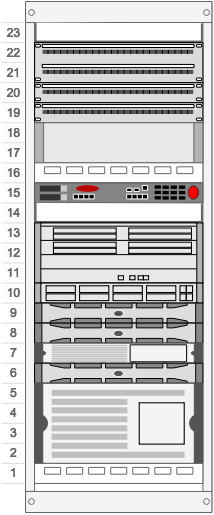
\includegraphics[]{fig2}
%	\caption{Exemplo de figura sem escala}
%	\label{fig2}
%\end{figure}

%Você pode rotacionar figuras também. Para isso utilize o parâmetro angle=-90. Repare que a escala da figura foi modificada pelo parametro height. Você também pode utilizar scale

%\begin{figure}
%	\centering
%	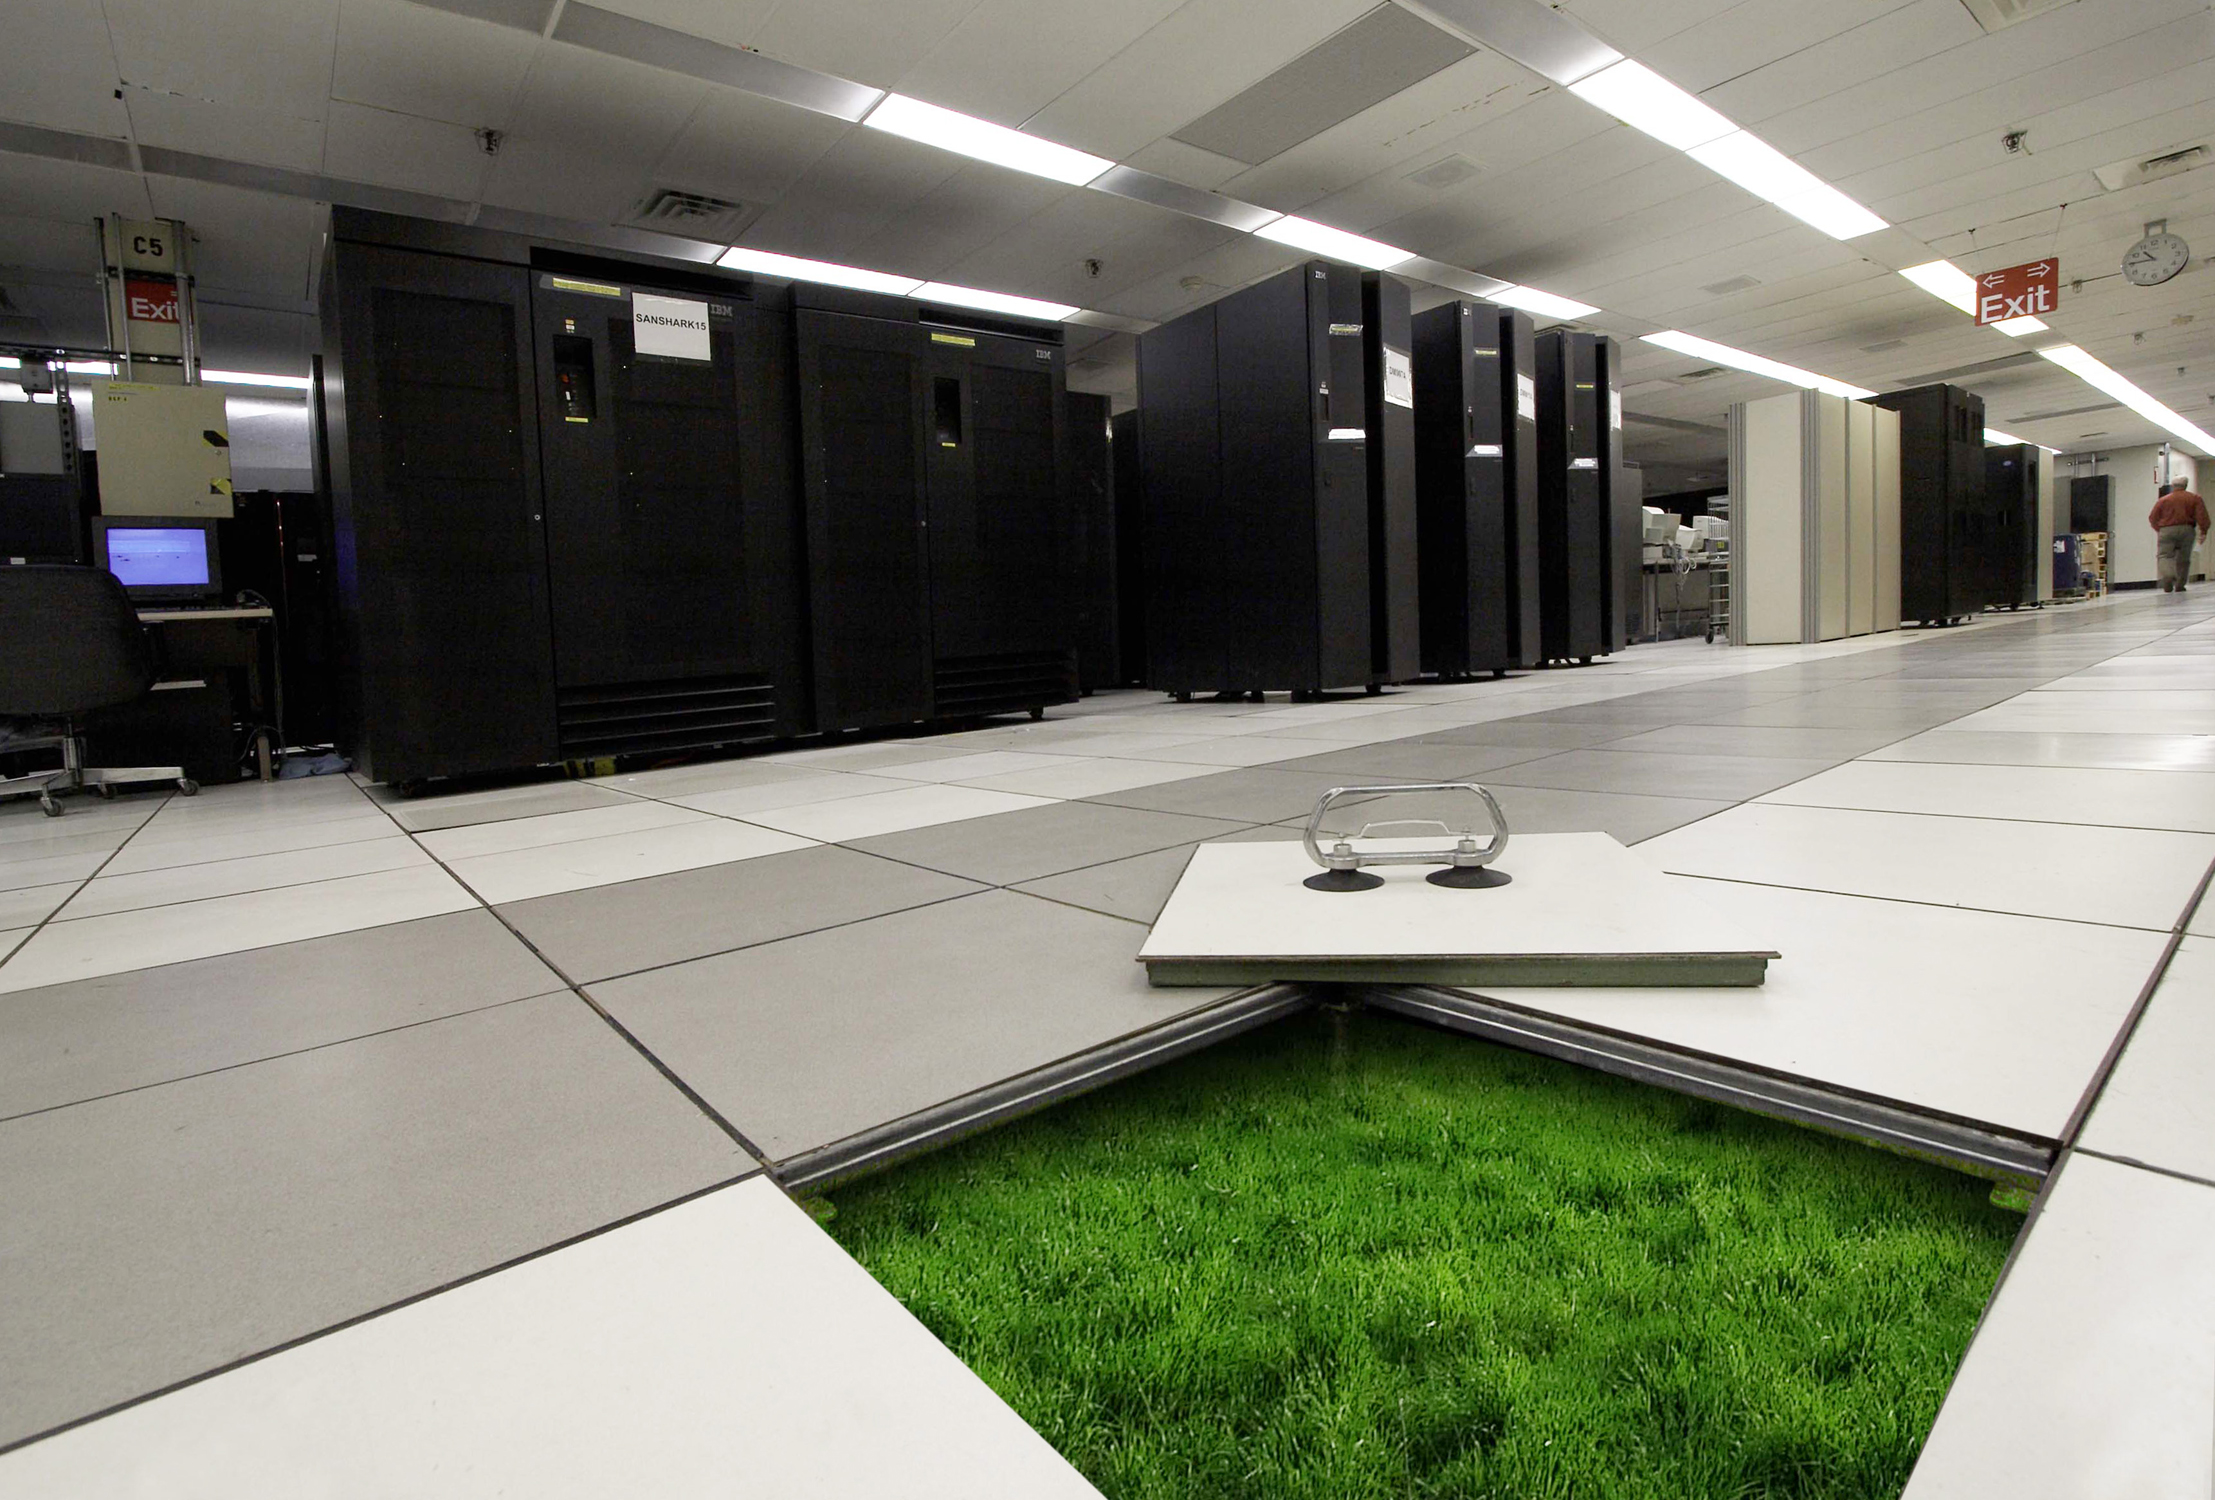
\includegraphics[height=\textwidth,angle=-90]{fig3}
%	\caption{Exemplo de figura rotacionada}
%	\label{fig3}
%\end{figure}


%% ***********************************************************************
%% === ate aqui    =====  ================================================
%% ***********************************************************************
\end{document}